%Cominezo del preambulo
%Definición del tipo dde docmentos y paquetes que se utilizaran
\documentclass[12pt,letterpaper]{article}
\usepackage[utf8]{inputenc}
\usepackage[spanish, es-tabla]{babel}
\usepackage{amsmath}
\usepackage{amsfonts}
\usepackage{amssymb}
\usepackage{makeidx}
\usepackage{graphicx}
\usepackage{lmodern}
\usepackage{kpfonts}
\usepackage[left=2cm,right=2cm,top=2cm,bottom=2cm]{geometry}


\spanishdecimal{.}

\makeindex
%fin del preambulo
\begin{document}
%\renewcommand{\tablename}{Tabla}
\renewcommand{\refname}{Bibliografía}


%definición de ccosas del documento como  fecha, autor etc.
\author{Ignacio Cabrera}
\title{Primear práctica escrita en \LaTeX}



\maketitle
%\tableofcontents
%\listoffigures
%\listoftables
\begin{abstract}


En está práctica se hizo bla bla bla bla bla bla bla bla bla bla bla bla bla bla bla bla bla bla bla bla bla bla bla bla bla bla bla bla bla bla bla bla bla bla bla bla bla bla bla bla bla bla bla bla bla bla bla bla bla bla bla bla bla bla bla bla bla bla bla bla bla bla bla bla bla bla bla bla bla bla bla bla bla bla bla bla bla bla bla bla bla bla bla bla bla bla bla bla
\end{abstract}


%Se comienza a escribir

% Se agrega una primera Sección
\section{Introducción}
\label{sec1}


Primer documento en  \LaTeX . \\
Este es un ejemplo.\\
Primera ecuación:
\begin{equation}
x= \dfrac{-b \pm \sqrt{b^{2}-4ac}}{2a} \texttt{Formula del chicharronero}
\end{equation}
segunda ecuación:

\begin{equation}
Ax^{2}+ Bx + C
\end{equation}

En el libro de \cite{2003fpp2.book.....H} definen el movimiento uniformemente acelerado como ...
 \\
 

En el libro \cite{1968fup..book.....A} se explica este movimiento como ... Siguiendo análisis hecho en \cite{1970AmJPh..38..781T} encontramos que ...

\section{Objetivo}
Más Bla bla bla

\section{Material}
El material utilizado para este experimento fue:
\begin{itemize}
\item 1 Flexómetro marca ... modelo ....
\item Cronómetro marca ...  modelo ...
\item Riel de Aire marca Pasco modelo ...
\item Cámara digital marca Fuji modelo ...
\end{itemize}
\section{Método experimental}

Para el experimento el equipo se monto como colocando el riel de aire ...\\
La cámara se colocó  en ...\\
Se determino que el tiempo sería la variable independiente y la distancia la variable dependiente.
\subsection{Observaciones}


Después de 10 deslizamientos nos dimos cuenta que el riel se movió y cambió la inclinación del ángulo en $1^{\circ}$
\section{Análisis de datos}

Para hacer toda la talacha se utilizó una computadora con un el software fulano o con el código hecho  por fulano para este análisis.\\
Primero se graficaron los datos ver gráficas \ref{gra1}, \ref{gra2} , \ref{gra3} y \ref{gra4}. 

%%%%%%%%%%%%%%%%%%%%%figura1%%%%%%%%%%%%%%%%%%%%%%%%%%%%
\begin{figure}[!h]

\begin{center}
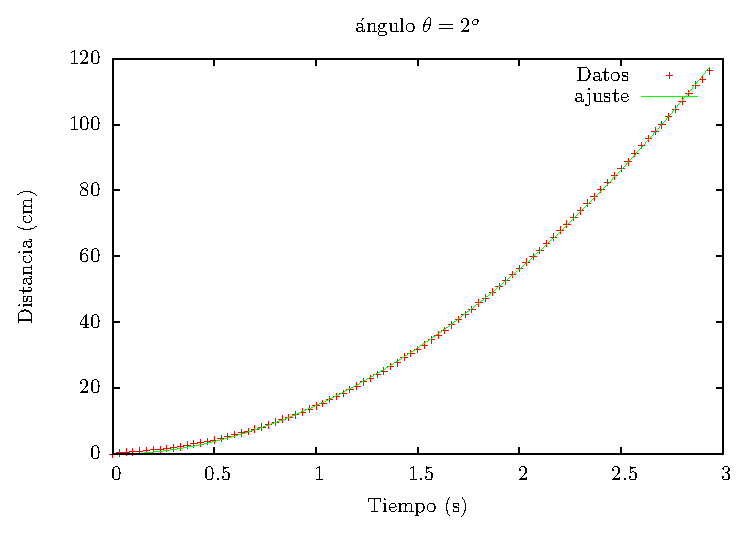
\includegraphics[scale=0.7]{grafica_out.eps} 
\caption{Gráfica 1. Plano inclinado con una pendiente de $\theta= 2^{o}$}\label{gra1}
\end{center}
\end{figure}
%%%%%%%%%%%%%%%%%%%%%%%%%%%%%%%%%%%%%%%%%%%%%%%%%%%%%%%%%
%%%%%%%%%%%%%%%%5figura 2%%%%%%%%%%%%%%%%%%%%%%%%%%%%%%%%%
\begin{figure}[!h]

\begin{center}
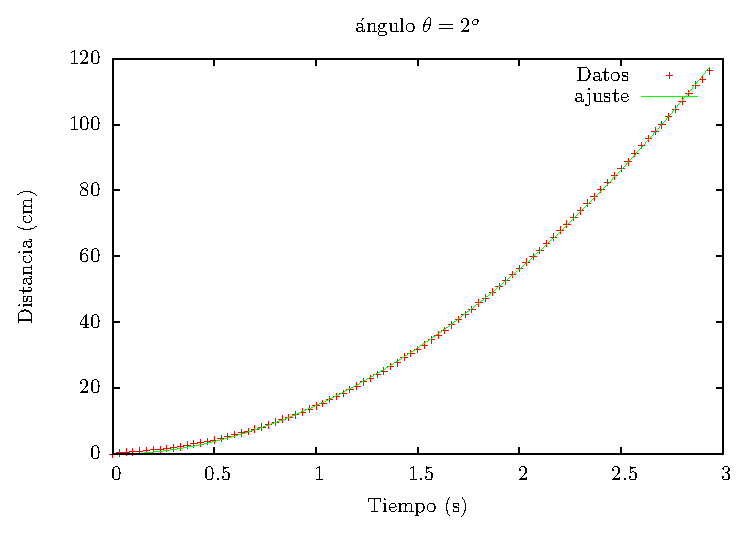
\includegraphics[scale=0.7]{grafica_out.eps} 
\caption{Gráfica 2. Plano inclinado con una pendiente de $\theta= 3^{\circ}$}\label{gra2}
\end{center}
\end{figure}
%%%%%%%%%%%%%%%%%%%%%%%%%%%%%%%%%%%%%%%%%%%%%%%%%%%%%%%%%%%%

%%%%%%%%%%%%%%%%%%%%%%figura3%%%%%%%%%%%%%%%%%%%%%%%%%%%%%%%
\begin{figure}[!h]

\begin{center}
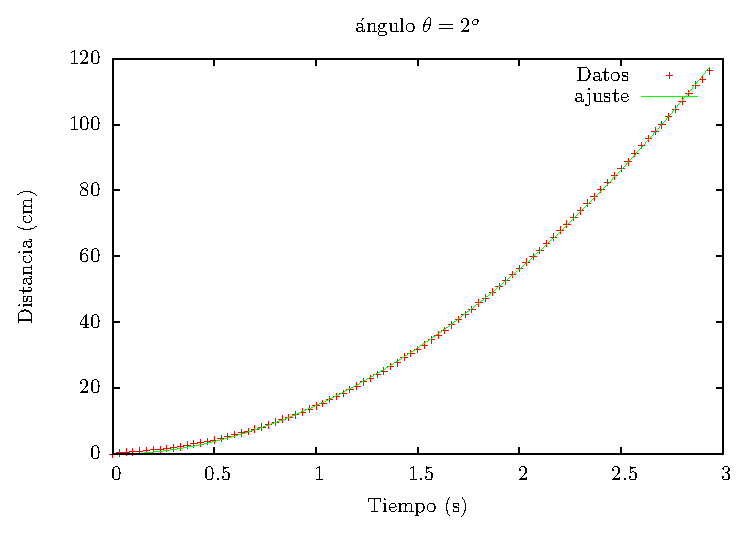
\includegraphics[scale=0.7]{grafica_out.eps} 
\caption{Gráfica 3. Plano inclinado con una pendiente de $\theta= 4^{\circ}$}\label{gra3}
\end{center}
\end{figure}
%%%%%%%%%%%%%%%%%%%%%%%%%%%%%%%%%%%%%%%%%%%%%%%%%%%%%%%%%%%%%%%%%%%%%%%%%%5

Se calculo el coeficiente de correlación de Pearson ($\rho$ para cada uno de los ángulos. Los valores se presentan en la tabla \ref{t1}.

%%%%%%%%%%%%%%%%%%%%%%figura3%%%%%%%%%%%%%%%%%%%%%%%%%%%%%%%
\begin{figure}[!h]

\begin{center}
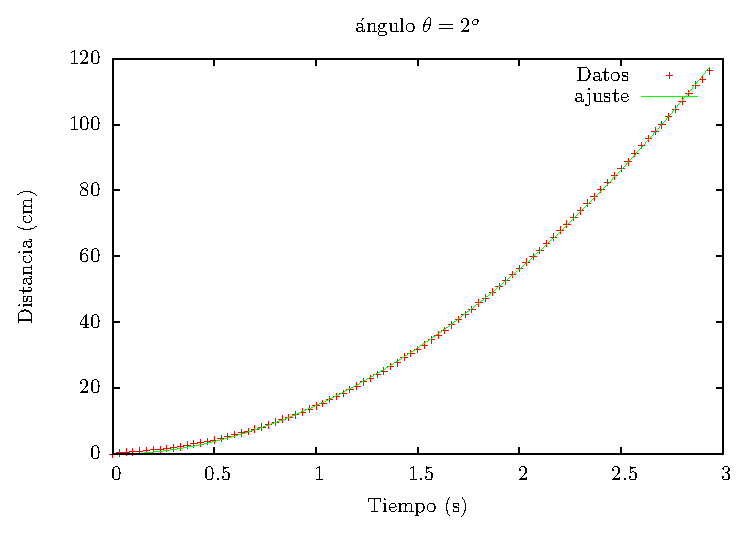
\includegraphics[scale=0.7]{grafica_out.eps} 
\caption{Gráfica 3. Plano inclinado con una pendiente de $\theta= 5^{\circ}$}\label{gra4}
\end{center}
\end{figure}
%%%%%%%%%%%%%%%%%%%%%%%%%%%%%%%%%%%%%%%%%%%%%%%%%%%%%%%%%%%%%%%%%%%%%%%%%%5


%%%%%%%%%%%%%%%%%%tabla1%%%%%%%%%%%%%%5
\begin{table}[!h]
\begin{center}
\begin{tabular}{cc}
\hline 
$\theta (^{\circ}) \pm 0.5 ^{\circ}$ &  $\rho$ \\ 
\hline
\hline 
2 & 0.87 \\ 
 
3 & 0.84 \\ 

4 & 0.85 \\ 

5 & 0.81 \\
\hline 
\end{tabular}
\caption{En esta tabla en la primera columna se presnrtan los valores del ángulo de inclinación de nuestro plano y en la segunda columna se presenta el vallor del coeficiente de correlación de los datos para cada ángulo. El coeficiente esá calulado en el plano líneal}\label{t1}
\end{center}
\end{table}
%%%%%%%%%%%%%%%%%%%%%%%%%%%%%%%%%%%%%%5

Después se tomo el logaritmo base 10 de los datos y se calculo el coeficiente de Pearson en el plano logarítmico, el resultado se presenta en la tabla \ref{tl}

%%%%%%%%%%%%%%%%%%tabla1%%%%%%%%%%%%%%5
\begin{table}[!h]
\begin{center}
\begin{tabular}{cc}
\hline 
$\theta (^{\circ}) \pm 0.5 ^{\circ}$ &  $\rho$ \\ 
\hline
\hline 
2 & 0.94 \\ 
 
3 & 0.92 \\ 

4 & 0.95 \\ 

5 & 0.91 \\
\hline 
\end{tabular}
\caption{En esta tabla en la primera columna se presnrtan los valores del ángulo de inclinación de nuestro plano y en la segunda columna se presenta el valor del coeficiente de correlación de los datos para cada ángulo utilizando el logritmo de los datos \textit{ie} en el plano logarítmico.}\label{tl}
\end{center}
\end{table}
%%%%%%%%%%%%%%%%%%%%%%%%%%%%%%%%%%%%%%5

Como el coeficiente de correlación es mejor en el plano logarítmico, se hacen los ajustes con mínimos cuadrados a una línea recta en el plano logarítmico (una ley de potencias en el plano lineal).

Los ajustes de los mínimos cuadrados a una recta en el plano logarítmico se presentan en la tabla \ref{tr}.

%%%%%%%%%%%%%%%%%%tabla1%%%%%%%%%%%%%%5
\begin{table}[!h]
\begin{center}
\begin{tabular}{ccccc}
\hline 
$\theta (^{\circ}) \pm 0.5 ^{\circ}$ &  m & $\delta$ m & b & $\delta$b \\ 
\hline
\hline 
2 & 1.93& 0.12 & 2.58 &  0.12\\ 
 
3 & 1.87& 0.13 & 2.64 & 0.14 \\ 

4 & 2.04& 0.10 & 2.76 & 0.11\\ 

5 & 1.89& 0.13 & 2.88 & 0.09 \\
\hline 
\end{tabular}
\caption{Resultados de ajustes de mínimos cuadrados para los 5 diferentes ángulos. la primera columna es el ángulo de incllinación, segunda columna el valor de la pendiente de la recta en el plano logarítmimco, tercetrra columna el errro de la pendiente, cuarta columna los valores de la ordenada al origen y la quinta columna es el errro de la ordenada al origen.}\label{tr}
\end{center}
\end{table}

Para evaluar los modelos, para cada uno de los ángulos se usa el criterio de la $ \chi_{red}^{2}$. Los valores de las  $ \chi_{red}^{2}$ para cada ángulo se presentan en la tabla \ref{xi}.

%%%%%%%%%%%%%%%%%%tabla1%%%%%%%%%%%%%%5
\begin{table}[!h]
\begin{center}
\begin{tabular}{cc}
\hline 
$\theta (^{\circ}) \pm 0.5 ^{\circ}$ &  $\chi_{red}^{2}$\\ 
\hline
\hline 
2 & 0.12\\ 
 
3 &  0.23\\ 

4 & 0.31\\ 

5 & 0.43\\
\hline 
\end{tabular}
\caption{Valores de las $\chi_{red}^{2}$ para los modelos para cada ángulo de inclinación. }\label{xi}
\end{center}
\end{table}

En la figura \ref{fm} se presentan los datos junto con el modelo

%%%%%%%%%%%%%%%%%%%%%%figura3%%%%%%%%%%%%%%%%%%%%%%%%%%%%%%%
\begin{figure}[!h]

\begin{center}
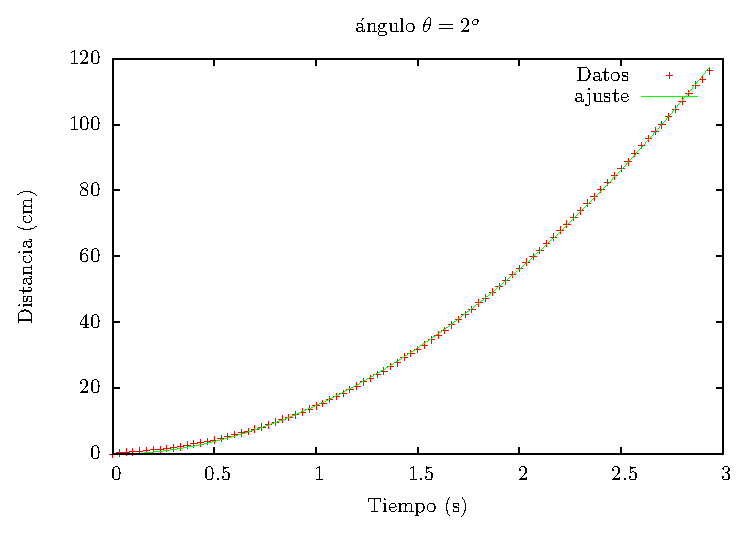
\includegraphics[scale=1]{grafica_out.eps} 
\caption{ángulo de inclinación de 2 grados y el modelo con los parámetros determinados por el método de mínimos cuadrados. La línea verde es el modelo y los puntos los datos con sus respectivos errores}\label{fm}
\end{center}
\end{figure}
%%%%%%%%%%%%%%%%%%%%%%%%%%%%%%%%%%%%%%%%%%%%%%%%%%%%%%%%%%%%%%%%%%%%%%%%%%5



\subsection{Observaciones}

EL conjunto de datos para el ángulo $\theta = 6 ^{\circ}$ no pudo utilizarse porque las escalas de medida no eran legibles en las imégenes de los videos. \\

Después del trabajo estadístico,  para todos los casos analizados se observa que la pendiente es $ \sim $ 2 y que el valor de la $\chi_{red}^{2}$ es cercano a cero, esto implica que el la dispersión de los datos es muy pequeña, y no se realizo ninguna manipulación de los datos para que este resultado se presente así. Por lo cual todos los modelos son bastante buenos.
%%%%%%%%%%%%%%%%%%%%%%%%%%%%%%%%%%%%%%5


\section{Resultados y conclusiones}\label{con}

En todos los ángulos se observa que la pendiente de las rectas en el plano logarítmico es $ \sim $ 2, este es un primer resultado, pues el experimento realizado esta mostrando que este es el comportamiento para el tipo de movimiento estudiado, bajo algunas condiciones.\\

Por otra parte el hecho de que los calores de la  $\chi_{red}^{2}$ sean tan pequeños nos dice que este modelo es muy acertado. Los resultados encontrados están en acuerdo con la ecuación del movimiento uniformemente acelerado, por lo cual se puede decir que las ecuaciones que describen dicho movimiento son validas mientras las velocidades sean pequeñas, no haya fricción o esta sea muy pequeña. \\

Mas Bla bla bla bla bla bla bla bla bla bla bla si se necesita.




\begin{thebibliography}{100}
\bibitem{2003fpp2.book.....H} Halliday, D., Resnick, 
R.,  \& Walker, J.\ 2003, Fundamentals of Physics, Part 2 (Chapters 12-20), by David Halliday, Robert Resnick, Jearl Walker, pp.~304.~ISBN 0-471-42962-7.~Wiley-VCH , December 2003.

\bibitem{1968fup..book.....A} Alonso, M., \& Finn, E.~J.\ 1968, Reading, Ma.: Addison-Wesley, 1968,

\bibitem{1970AmJPh..38..781T} Tipler, P.~A., \& Dexter, R.~N.\ 1970, American Journal of Physics, 38, 781 

\end{thebibliography}
  

bla bla bla

Aquí termina la primera práctica escrita en \LaTeX.
\end{document}